% !TEX program = pdflatex
% !BIB program = biber

%% One can optionally have all this inside a separate setup.tex
% !TEX program = pdflatex
% !BIB program = biber

% !TEX root = main.tex
\documentclass[10pt, a4paper]{report}
% \documentclass[12pt, a4paper, oneside]{memoir}
% \chapterstyle{veelo}

%% Sets page size and margins
\usepackage[a4paper,top=3cm,bottom=2cm,left=3cm,right=3cm,marginparwidth=1.75cm]{geometry}
%\usepackage[left=2cm,top=2cm,bottom=2cm,bindingoffset=1cm]{geometry}

\usepackage[utf8x]{inputenc}
\usepackage{graphicx}
\usepackage{float}
\usepackage{imakeidx}
\usepackage{amsmath}
\usepackage[colorlinks=true, allcolors=blue]{hyperref}
\usepackage{graphicx}
\usepackage{float}
\usepackage{imakeidx}
\usepackage{amsmath}
\usepackage{url}
\usepackage[export]{adjustbox}
\usepackage{subcaption}
\usepackage[toc,page]{appendix}

%% Useful packages
\usepackage[colorinlistoftodos]{todonotes}
\usepackage[T1]{fontenc}

%% Language and font encodings
\usepackage[english]{babel}

%% Define a few colours to be used throughout the document
\usepackage{tikz,xcolor}
\definecolor{TextColor}{HTML}{000000}
\definecolor{SideColorDark}{HTML}{000000}
\definecolor{MainColor}{HTML}{0000FF}
\definecolor{OppositeColor}{HTML}{FF0000}
\definecolor{HighlightColor}{HTML}{FFFF00}


%% Code block style
%  Load the \ttfamily font
\usepackage[T1]{fontenc}
\usepackage[scaled]{beramono}

%  Format code blocks
\usepackage{listings}
%  Change caption name
\renewcommand*{\lstlistingname}{Code block}
\captionsetup[lstlisting]{margin=0cm,format=hang,font=small,format=plain,labelfont={bf,up},textfont={it}}
%  Style
\lstset{
  showstringspaces=false,
  formfeed=\newpage,
  commentstyle=\itshape,
  backgroundcolor=\color{gray!5},
  breakatwhitespace=false,         % sets if automatic breaks should only happen at whitespace
  breaklines=true,                 % sets automatic line breaking
  captionpos=b,                    % sets the caption-position to bottom
  commentstyle=\color{gray},    % comment style
  escapeinside={\%*}{*)},          % if you want to add LaTeX within your code
  keepspaces=true,
  numbersep=2mm,                   % how far the line-numbers are from the code
  showspaces=false,
  showstringspaces=false,
  showtabs=false,
  stepnumber=1, numberfirstline=false,
  basicstyle=\linespread{1}\footnotesize\ttfamily,
  keywordstyle=\bfseries\color{MainColor},
  stringstyle=\itshape\color{OppositeColor},
  numberstyle=\footnotesize\ttfamily\color{gray},
  numbers=left,xleftmargin=4mm,framexleftmargin=0mm,xrightmargin=0mm,
  frame=top,frame=bottom,
}

\title{Insert title here}
\author{Daniel Robinson\\18361137}

\begin{document}
% \maketitle
    \begin{titlepage}
        \begin{center}
            \vspace*{1cm}
            
            \begin{figure}
			\centering
            
\includegraphics[scale=2]{images/UScrest-top.jpg}
            \end{figure}
            
            \huge
            \textbf{Normalized Differential Vegetation Index Mapping}

            \large            
            \vspace{2.5cm}

            \textbf{Daniel Robinson\\18361137}

            \vspace{2.5cm}    
            
            \textbf{Report submitted in partial fulfilment of the requirements of the module Project (E) 448
            for the degree Baccalaureus in Engineering in the Department of Electrical and Electronic
            Engineering at the University of Stellenbosch}
            
            \vspace{4cm} 
            
            \textbf{STUDY LEADER: Corné van Daalen\\DATE: November 2017}
            
            
        \end{center}
\end{titlepage}

\newpage
\section{Acknowledgements}
\section{Declaration of own work}

I, the undersigned, hereby declare that the work contained in this report is my own original work
unless indicated otherwise.\\\\

\noindent
Signature: \underline{ }\underline{ } Date: \underline{ }\underline{ }

\section{Summaries}
\subsection{English}
\subsection{Afrikaans}

\tableofcontents
\listoffigures
\listoftables

\newpage

% \begin{abstract}
% Your abstract.
% \end{abstract}

\section{Project Overview}

In this section the project objectives and requirements are specified.

\subsection{Project Objectives}
In order to be deemed successful the project needs to satisfy the following:

\begin{itemize}
    \item Investigate observable parameter(s) beneficial to agriculture within large areas
\end{itemize}

\subsection{Means}

\begin{itemize}
    \item Develop an observation platform to map areas from height (NADIR)
    \item Determine observation equipment
    \item Process sampled data and draw conclusions
    \item Develop control tests to verify / prove conclusions
\end{itemize}

\subsection{Why}

There's currently a water shortage crisis in South Africa, and in other parts of the world, potentially due to global warming. One of the sectors that it affects is agriculture. Farmers may be using less water on their crops, or load sharing. There's also the case of human error, where incorrect amounts of water or fertilizer (for example) is used. Lastly, plant disease is also a problem.\\

To mitigate such problems, farmers would physically observe or sample their produce from the ground. It can be a time consuming task, and if sensor data is used, a mass of hand-held readings can prove complex. Perhaps a simpler, large-scale method of observing such changes can be used.

\section{Setup}

\subsection{Raspberry Pi}
\subsection{Building Drone}

\begin{figure}
\centering
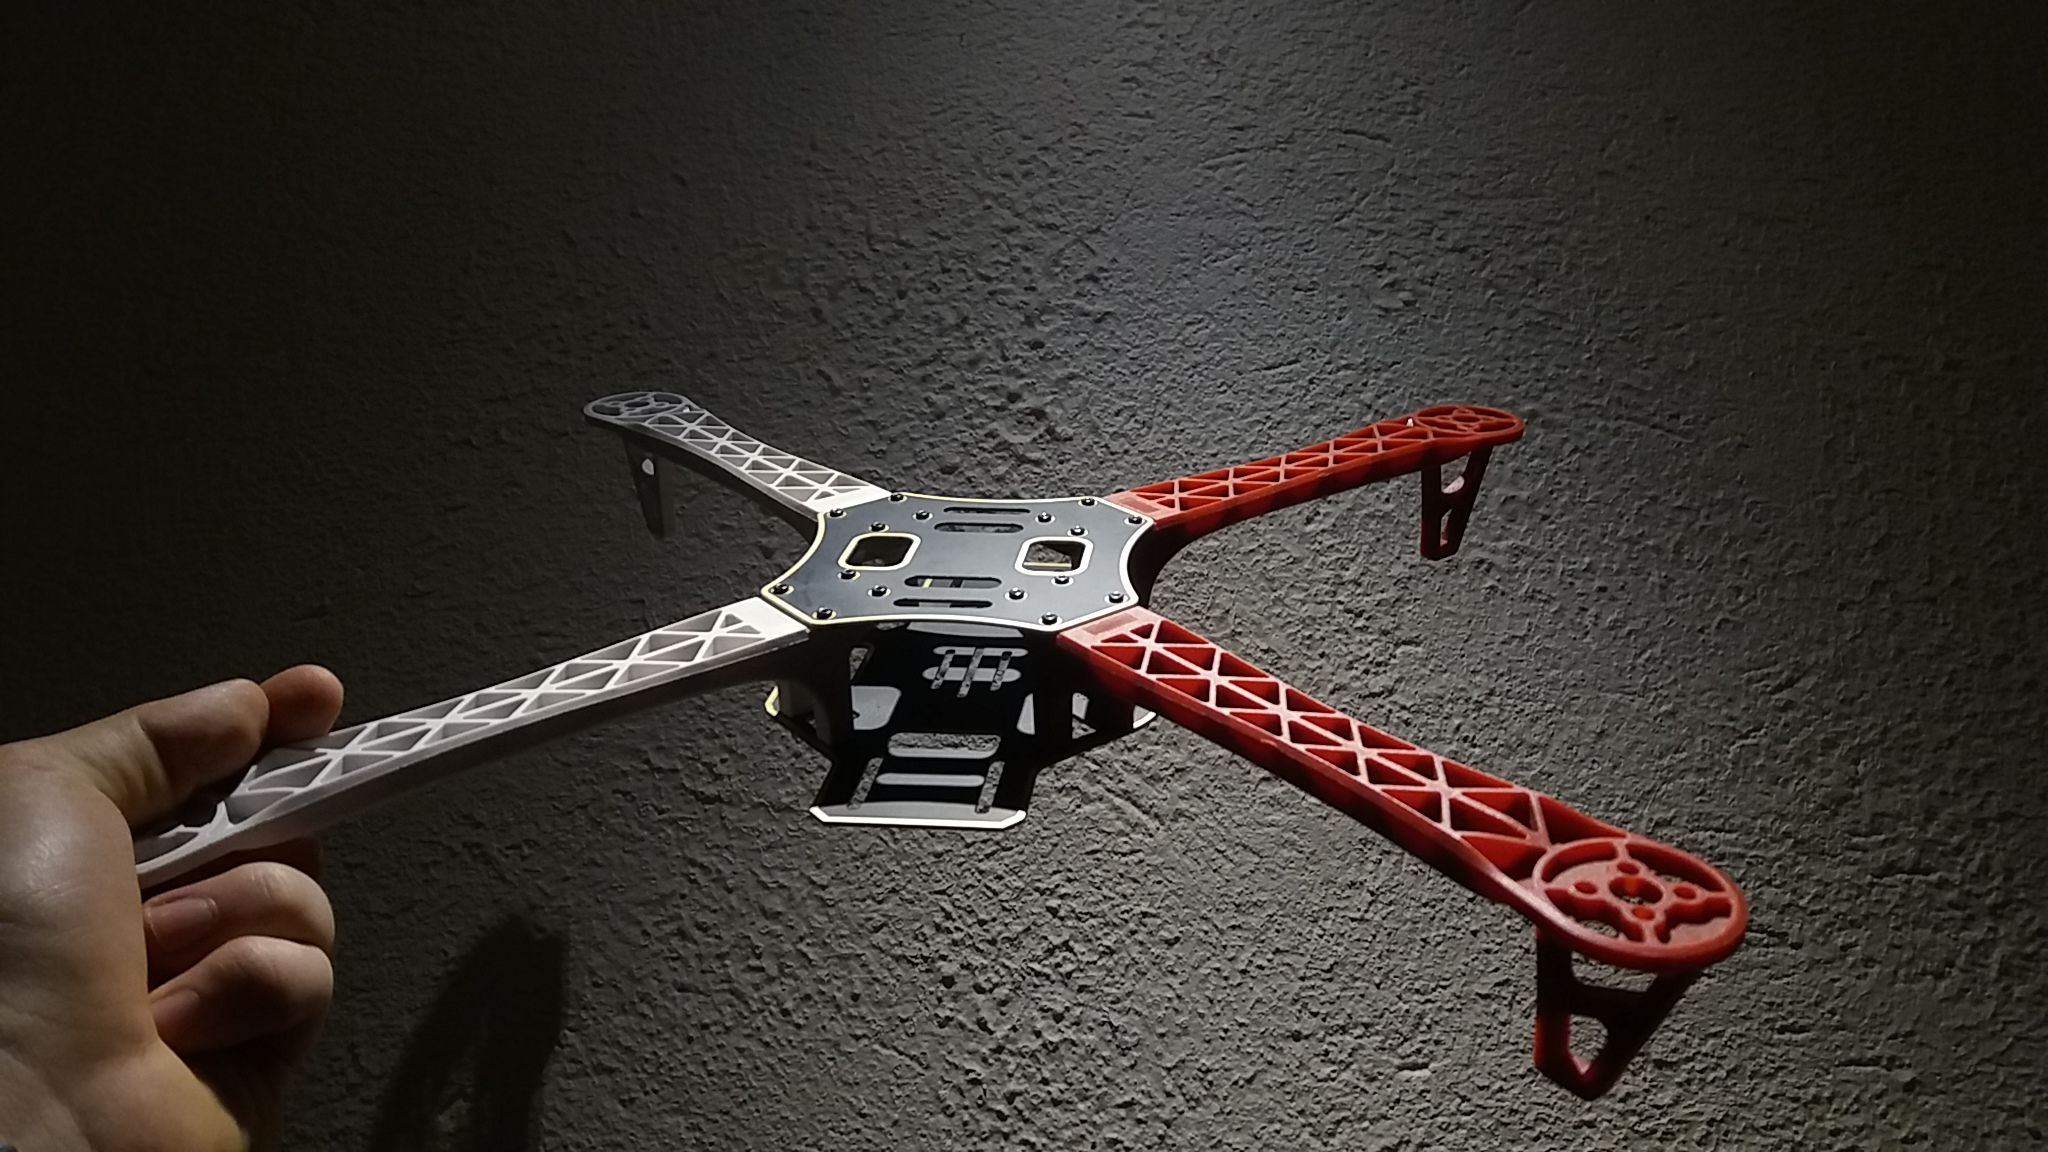
\includegraphics[scale=0.1]{images/drone-build-frame.jpg}
\caption{F450 frame
}% Reproduced from \cite{gopher}}
\label{fig:frame}
\end{figure}


% \begin{figure}[H]
% \begin{subfigure}{0.5\textwidth}
% \includegraphics[scale=0.3]{3.png}
% \caption{Pushbutton Switch.\\
% Reproduced from \cite{cpi}.}
% \label{fig:p}
% \end{subfigure}
% \begin{subfigure}{0.5\textwidth}
% \centering
% \includegraphics[scale=0.1]{2.png}
% \caption{InvenSense MPU-9250.\\
% Reproduced from\cite{iven}.}
% \label{fig:att}
% \end{subfigure}
% \begin{subfigure}{0.5\textwidth}
% \centering
% \includegraphics[scale=0.3]{1.png}
% \caption{Altimeter Module MS5607.\\ Reproduced from \cite{par}.}
% \label{fig:pres}
% \end{subfigure}
% \caption{Sensors}
% \label{fig:sensors}
% \end{figure}


% In order for the data to be transmitted successfully, it needs to be in a format acceptable by the GCS. The data will be stored in a JSON packet created using a C++ library\cite{ajson}.

% Code block \ref{code:json1} shows a potential data packet.

% \lstset{language=html,caption={Potential packet},label=code:json1}
% \begin{lstlisting}
% {
%   "temperature": "11.3",
%   "pressure": "99.325"
% }
% \end{lstlisting}

% \begin{figure}
% \centering
% \includegraphics[scale=0.35]{flight_path.png}
% \caption{CanSat flight trajectory\\
% Reproduced from \cite{gopher}}
% \label{fig:flight_path}
% \end{figure}




% \subsection{How to add Tables}

% Use the table and tabular commands for basic tables --- see Table~\ref{tab:widgets}, for example. 

% \begin{table}
% \centering
% \begin{tabular}{l|r}
% Item & Quantity \\\hline
% Widgets & 42 \\
% Gadgets & 13
% \end{tabular}
% \caption{\label{tab:widgets}An example table.}
% \end{table}

% \subsection{How to write Mathematics}

% \LaTeX{} is great at typesetting mathematics. Let $X_1, X_2, \ldots, X_n$ be a sequence of independent and identically distributed random variables with $\text{E}[X_i] = \mu$ and $\text{Var}[X_i] = \sigma^2 < \infty$, and let
% \[S_n = \frac{X_1 + X_2 + \cdots + X_n}{n}
%       = \frac{1}{n}\sum_{i}^{n} X_i\]
% denote their mean. Then as $n$ approaches infinity, the random variables $\sqrt{n}(S_n - \mu)$ converge in distribution to a normal $\mathcal{N}(0, \sigma^2)$.


% \subsection{How to create Sections and Subsections}

% Use section and subsections to organize your document. Simply use the section and subsection buttons in the toolbar to create them, and we'll handle all the formatting and numbering automatically.

% \subsection{How to add Lists}

% You can make lists with automatic numbering \dots

% \begin{enumerate}
% \item Like this,
% \item and like this.
% \end{enumerate}
% \dots or bullet points \dots
% \begin{itemize}
% \item Like this,
% \item and like this.
% \end{itemize}

% \subsection{How to add Citations and a References List}

% You can upload a \verb|.bib| file containing your BibTeX entries, created with JabRef; or import your \href{https://www.overleaf.com/blog/184}{Mendeley}, CiteULike or Zotero library as a \verb|.bib| file. You can then cite entries from it, like this: \cite{greenwade93}. Just remember to specify a bibliography style, as well as the filename of the \verb|.bib|.

% You can find a \href{https://www.overleaf.com/help/97-how-to-include-a-bibliography-using-bibtex}{video tutorial here} to learn more about BibTeX.

% We hope you find Overleaf useful, and please let us know if you have any feedback using the help menu above --- or use the contact form at \url{https://www.overleaf.com/contact}!

\newpage
\bibliographystyle{plain}
% \bibliographystyle{alpha}
\bibliography{references}

\end{document}